%%%%%%%%%%%%%%%%%%%%%%%%%%%%%%%%%%%%%%%%%%%%%%%%%%%%%%%%
% E W Fulp  2/2/2014 (CSC 790 Project 1)
%
%%%%%%%%%%%%%%%%%%%%%%%%%%%%%%%%%%%%%%%%%%%%%%%%%%%%%%%%
\documentclass[10pt]{article}

\usepackage[dvips]{color}
\usepackage{fancybox}
\usepackage{latexsym}
\usepackage{fancyhdr}
\usepackage{subfigure}
\usepackage{epstopdf}
\usepackage{slashbox}
\usepackage{amsfonts,amssymb,latexsym}
\usepackage{amsthm}  % used to make "proof" work
\usepackage{graphicx}
\usepackage{enumerate}
\usepackage{amsmath}  % added later
%\usepackage{setspace} % added later
\usepackage{color}    % added later
\everymath{\displaystyle} % added later
\usepackage{float}
\usepackage{tikz} % added later

 \textwidth=6.5in
 \oddsidemargin=0in
 \evensidemargin=0in
 \topmargin=-0.25in
 \headsep=0in
 \headheight=0in
 \textheight=9.5in

\newcommand{\Questions}[1]{
\subsection*{Questions {\rm \normalsize (\textsf{\textit{#1 points}})}}
}

\pagestyle{fancy}
\rhead{}\chead{}\lhead{}
\renewcommand{\headrulewidth}{0pt}
\renewcommand{\footrulewidth}{0.4pt}
\cfoot{\shortstack{\textit{\textsf{\footnotesize CSC 790}} \\
\textit{\textsf{\footnotesize Spring 2014}} \\ \thepage}}


\begin{document}
\newcommand{\dis}{\displaystyle}
\newcommand{\beq}{\begin{eqnarray}}
\newcommand{\eeq}{\end{eqnarray}}


{
 \setlength{\tabcolsep}{0in}
 \noindent
 \begin{tabular*}{\textwidth}{p{5.0in}r}
 \begin{tabular}{l}
 \Large \textbf{CSC 790 A: Project 1} \\
 \Large \textbf{Deception Game} v1.0 \\ \\
 \end{tabular}
 &
  {\renewcommand{\arraystretch}{1.25}
  \setlength{\tabcolsep}{0.1in}
  \begin{tabular}{|l|} \hline
    \textbf{\textsf{Due}} \\ \hline \hline
    \textit{\textsf{12:30pm Thursday, 2/20}} \\ \hline
  \end{tabular}} \\ \\ \hline \hline
\end{tabular*}
}

\section*{Project Description}

\thispagestyle{fancy}

As discussed in class, deception conceals or obscures an entity's existence or attributes so to  intentionally mislead adversaries. Several deception methods for computer systems have been developed and researched; examples include address hopping/shuffling, honeypots,  and honeynets. One aspect of deception that has not been fully considered is the deployment and subsequent management of these methods.  For example given a computer network to protect, what type of deception is best? How often should address shuffling be performed? What is the minimum number of honeypots required to be effective? Will address shuffling and honeypots in combination provide better security? For this project you will develop a mathematical model to analyze the performance of deception to better understand  deployment and management. In other words, the best defense strategies for a set of defense and attacker options.

\section*{Network and Attacker Description}

Assume you are the administrator of a computer network consisting of vulnerable computers (like Fletcher's), secure computers, and empty addresses. The attacker seeks to map your network and find the vulnerable computers using a \textit{scan} which may or may not be followed by an \textit{exploit attempt}. Instead of using specific amounts for the number addresses, number of computer, etc... use  variables. We're creating models after all.

\begin{itemize}
   \item There are $n$ total addresses available to the administrator.
   \item There are $m$ computers in the network, of which $v$ are vulnerable; therefore $v \leq m \leq n$.
   \item The attacker is aware of the address space $n$ and seeks to find at least  $\alpha$ percent of the $v$ vulnerable computers; therefore, $0 < \alpha \leq 1$.
   \item The attacker will try $k$ scans of the network to find vulnerable systems.
\end{itemize}

\section*{Available Deception Techniques}

Several deception techniques are possible, however this assignment will only consider address shuffling and honeypots. Furthermore to help analysis you can ignore some implementation details however you will still need to consider the revenue and costs (administrative and attacker) of each technique. Revenue and costs are difficult to quantify. Identifying the cost of deployment is possible, although there are fixed costs, variable costs, ... \textit{What is the administrative revenue associated with a successful defense?} \textit{What is administrative the cost of a failed defense?} One possible solution is to consider utility instead of actual monetary amounts.

\subsection*{Address Shuffling}

Address shuffling (or hopping, I can't decide) simply replaces a system's IP address with another. Once this occurs attacker reconnaissance information becomes invalid. An important administrative cost to consider is the loss of legitimate connections.

\subsection*{Honeypots}

Honeypots are systems designed to detect unauthorized access. The system mimics an actual computer server and can record the source of an attacker (IP address) and type of exploit. As a result attackers seek to avoid these systems (so there is a high attacker cost). There is also a nontrivial administrative cost associated deploying and managing honeypots.

\section*{Models and Games}

As previously described, you will develop mathematical models of defense strategies for a computer network. Such models are very useful for predicting the performance of a system that cannot be easily tested empirically. Verifying the model with empirical results an important, and necessary step, but will not be done for this assignment.

\textit{What type of model should you consider?}  We are interested in the likelihood of attacker success and given the amount of chance associated with a scan, probabilistic models are probably best suited. For example the NASR paper modeled the probability of attacker success as $\frac{v}{n}$, which is the probability that attacker will randomly scan one of the $v$ vulnerable machines\footnote{In all fairness, the NASR paper defended against hitlist attacks, so there were no scans and as a result their simple model is correct. But how was the list acquired? }. This is a start, but this simple equation does not take into account $k$ scans are probably performed. Specifically each scan can provide the attacker knowledge (for example, whether or not to attempt the address again). If no defense is provided and the attacker can attempt $n$ scans, then the probability that the attacker will find $v$ vulnerable computers is 1. The NASR model does not directly provide this insight.

Developing the probability equations for different scenarios is possible, but perhaps a better approach would associate another known model with the network system. \textit{Can the system be modeled as a dice game?} Selecting a computer to scan (attackers point of view) could be modeled as rolling a $n$ sided die, where each side represents an address. Consider the implication of shuffling and how that would map to a dice game. \textit{Can the system be modeled as a card game, a roulette wheel, keno game\footnote{Maybe not keno, as according to Cody, you never lose in keno.}, ...?}  Using these known models an equation for the attacker success probability can be determined, \textit{I think.}  I hope you will select one model for all the defense strategies.

\subsection*{Applying a Bad Introduction to Game Theory}

This project is interested in determining the best defense strategy given a set of attacker strategies. As such, game theory is best suited for determining the best strategies if they are described mathematically (the point of the previous section). You will consider the system  as a two player (administrator and attacker), non-cooperative, competitive game.

\subsubsection*{Player Actions, Payoffs, and Best Strategies}

Using game theory you must define the actions (strategies) available to each player. For example depending on the question asked in the assignment, the administrator could have the following strategies: do nothing, address shuffling, or honeypot. The attacker may have the option to do nothing, scan, or scan and attempt exploit. Using this information a \textit{payoff} matrix can be developed where the matrix entries are the payoff values for the defender and attacker.  An example payoff matrix is given below.

\begin{center}
\renewcommand{\arraystretch}{1.25}
\begin{tabular} {|c|c|c|c|} \hline
 \backslashbox{Attacker}{Admin} & Static (no deception) & Shuffle & Honeypot  \\ \hline
  Scan & $(E^{d}_{s}, E^{a}_ {s})$ & $(E^{d}_{sh}, E^{a}_{s})$ & $(E^{d}_{h}, E^{a}_{s})$ \\ \hline
  Scan \& Attack & $(E^{d}_{s}, E^{a}_{a})$ & $(E^{d}_{sh}, E^{a}_{a})$ & $(E^{d}_{h}, E^{a}_{a})$ \\ \hline
\end{tabular}
\end{center}

\noindent
The values $E^{i}_{j}$ is the expected payoff for player $i$ using strategy $j$, for example $E^{d}_{s}$ is the expected payoff for the defender using static addressing. This value is dependent on the attacker success probability and can be calculated as
\[
  E^{d}_{s} = (1 - \beta_{s}) \cdot r_{s} - \beta_{s} \cdot c_{s}
\]
where $\beta_{s}$ is the probability the attacker is successful given a static defense, $r_{s}$ is the revenue of the defense, and $c_{s}$ is the cost of the defense. The remaining expected payoffs can be determined in a similar fashion. Using the completed matrix the best strategies (dominate, Nash-equilbria) can be found, \textit{I hope}.

\vfill
\newpage

\section*{Project Requirements}

The deliverable for this project will be a report describing your model (probabilistic and game) and your answers to the following sections. Your report must be written succinctly and neatly (yes, typeset).

\section{Static Addressing}

Develop a model to analyze static addressing which is equivalent to no defense. An important part of the model will be the probability of attacker success ($\beta$) for finding at least $\alpha$ percent of $v$ vulnerable computers in a network of $n$ addresses and $m$ computers total given $k$ attacker scans. Yes, a lot of variables to consider.

\Questions{15}
You must correctly answer the following questions to receive full credit for this part of the project.
\begin{enumerate}
  \item What is the equation for attacker success ($\beta$) for static addressing? Describe the equation and how it correctly models the system.
  \item Assume the attacker only needs to find one vulnerable machine. Graph the attacker success rate as the number of scans ($k$) increases given a  \textbackslash 16 (class B) network, where 25\% of the addresses have machines and 10\% of these machines are vulnerable. Comment on your results.
    \item Provide a 3-D graph of the attacker success rate (z-axis) as the number of scans ($k$, x-axis) and attacker find percentage increases ($\alpha$, y-axis). Assume a  \textbackslash 16 (class B) network, where 25\% of the addresses have machines and 10\% of these machines are vulnerable. Comment on your results.
\end{enumerate}

\section{Address Shuffling}

Develop a model for address shuffling where all $n$ addresses are shuffled. An important part of the model will be the probability of attacker success ($\beta$) for finding $\alpha$ percent of $v$ vulnerable computers. Again, the a network consists of $n$ addresses and $m$ computers, and the attacker can perform $k$ scans. In addition your model should consider the frequency of shuffling denoted as $\gamma$.

Shuffling frequency does imply a temporal component to the model, which is a non-trivial addition. To simplify your initial analysis, you can consider the frequency to be associated with the scan attempts instead of over fixed time intervals (although you can use intervals if you like, \textit{it might be easier}). Therefore $0 \leq \gamma \leq 1$ where $\gamma = 0$ is static addressing and $\gamma = 1$ is \textit{perfect shuffling} which means the addresses are shuffled after each scan attempt. Therefore with \textit{perfect shuffling} given $k$ scans, $k$ shuffles would occur which provides the best shuffle defense but has a very high cost.

\Questions{25}
You must also correctly answer the following questions to receive full credit for this part of the project.
\begin{enumerate}
  \item What is the equation for attacker success ($\beta$) for perfect address shuffling? Describe the equation and how it correctly models the system.
  \item Assume the attacker only needs to find one vulnerable machine and the system is defended with perfect shuffling. Graph the attacker success rate as the number of scans ($k$) increases given a  \textbackslash 16 (class B) network, where 25\% of the addresses have machines and 10\% of these machines are vulnerable. Compare with static addressing and comment on your results.
  \item What is the equation for attacker success ($\beta$) for shuffling with frequency $\gamma$? Describe the equation and how it correctly models the system.
    \item Provide a 3-D graph of the attacker success rate (z-axis) as the number of scans ($k$, x-axis) and shuffling frequency increases ($\gamma$, y-axis). Assume a  \textbackslash 16 (class B) network, where 25\% of the addresses have machines, 10\% of these machines are vulnerable, and the attacker is required to find at least 25\% of the vulnerable computers. Comment on your results.
    \item An interesting question is how many of the addresses should be shuffled. Would only shuffling vulnerable machines with empty addresses provide the same protection as shuffling the entire network? Defend your position, graphs can help the argument.
\end{enumerate}

\section{D-Quan's Dance Groves and Address Shuffling}

Researchers from UNCC created a MT system that relies on Software Defined Networks (SDN) to provide a MT defense. One requirement of their approach is that computers must hop/shuffle in a subnet (which is a portion of the complete network). For this part of the assignment, you will create a model of this approach to determine the defense performance, then compare it to a more traditional notion of address shuffling (defined in the previous section).

Assume the address space consists of $n$ addresses and are divided into $s$ equal subnets. In addition, assume that each subnet will consist of the same number of computers, $\frac{m}{s}$, and vulnerable $\frac{v}{s}$ per subnet, where $m$ and $v$ are multiples of $s$ (so everything divides evenly). Develop a model for subnet address shuffling where all $n$ addresses are shuffled. An important part of the model will be the probability of attacker success ($\beta$) for finding $\alpha$ percent of $v$ vulnerable computers. Again, the attacker can perform $k$ scans. In addition your model should consider the frequency of shuffling denoted as $\gamma$.

\Questions{15}
You must also correctly answer the following questions to receive full credit for this part of the project.
\begin{enumerate}
  \item What is the equation for attacker success ($\beta$) for D-Quan's perfect address shuffling? Describe the equation and how it correctly models the system.
  \item Assume the attacker only needs to find one vulnerable machine and the system is defended with perfect shuffling. Graph the attacker success rate as the number of scans ($k$) increases given a  \textbackslash 16 (class B) network, where 25\% of the addresses have machines and 10\% of these machines are vulnerable. Compare with static addressing and traditional (no subnet) shuffling, then comment on your results.
  \item Is this method better, worse, or the same as traditional shuffling? Are your results consistent with the results reported in the UNCC paper?

\end{enumerate}


\section{Honeypot}

Develop a model for honeypots. In this system the attacker must avoid honeypots, if a honeypot is contacted the attack must stop (very high cost to the attacker). Therefore an important part of the model will be the probability of attacker success ($\beta$) for finding $\alpha$ percent of $v$ vulnerable computers using $k$ scan without contacting any honeypots. This will depend on the number of honeypots deployed which will be denoted as $h$, where $m+h \leq n$.

\Questions{30}
You must also correctly answer the following questions to receive full credit for this part of the project.
\begin{enumerate}
  \item What is the equation for attacker success ($\beta$) for $h$ honeypots? Describe the equation and how it correctly models the system.
  \item Assume the attacker only needs to find one vulnerable machine and the system is defended with honeypots. Graph the attacker success rate as the number of honeypots ($h$) increases given a  \textbackslash 16 (class B) network, where 25\% of the addresses have machines, 10\% of these machines are vulnerable, and the attacker is allowed to scan 10\% of the network. Compare with no defense and shuffling, then comment on your results.
    \item Provide a 3-D graph of the attacker success rate (z-axis) as the number of scans ($k$, x-axis) and number of honeypots increases ($h$, y-axis). Assume a  \textbackslash 16 (class B) network, where 25\% of the addresses have machines, 10\% of these machines are vulnerable, and the attacker is required to find at least 25\% of the vulnerable computers. Comment on your results.
\end{enumerate}

\section{Shuffle or Honeypots}

The probabilities of success for the different defenses can be used to determine the expected payoffs, and complete the payoff matrix. The matrix can then identify the best defense (or attack) strategy given the alternatives. As described earlier, an important part for developing the matrix will be to identify utility values for defenses and attacks. Using a generic security credit, instead of \texttt{US AMERICAN DOOLARS}, can simplify this process. If you decide to take this approach you will need to justify the various values associated with deploying defenses, attempting an attack, attacker success, and defender loss, etc...

\Questions{15}
You must also correctly answer the following questions to receive full credit for this part of the project.
\begin{enumerate}
  \item Assign revenue and cost variables for the different attacks and defenses, then determine the payoff equations and complete the matrix.
  \item Make realistic assumptions about the comparative revenue and costs (for example shuffling is less expensive than honeypots) and determine the best strategies. Comment on your results, note graphs help.
\end{enumerate}


\section*{Solutions}
\subsubsection*{1.1}

In this mathematical model, we need to assume that $\alpha v$ is an integer and $ k \geq \alpha v$.

\noindent So, the whole question is equivalent to this: consider that there are $n$ candy boxes in total (the IP address space), $m$ of which have candies inside (each box contains either only one candy or is empty). There are two kinds of candies among them, the red ones (the vulnerable computers, with the number $v$) and the green ones (the secure computers, with the number $m-v$). Now, a boy randomly picks $k$ boxes and only those red candies can meet his interest because he is so naughty (attacker), so those boxes contain green candies are the same with those empty boxes to him (IP addresses associated with secure computers and no computers are the same to the attacker). His choice space is $n \choose k$, suppose $x (0 \leq x \leq k)$ of his picks have red candies, then the target space is $v \choose x$$ n-v \choose k-x$. To make this naught boy happy, there must be at least $\alpha v$ red candies, thus the possibility $\beta$ that he is happy (attacker success) is:
\beq
\beta &=& \sum\limits_{x=\alpha v}^{\min{(k,v)}} \frac{{v \choose x}{n-v \choose k-x}}{{n \choose k}}. \nonumber
\eeq

\subsubsection*{1.2}
Here, $n = 2^{16}-2 = 65534$, $m=\frac{n}{4} = 16383.5$, $v = \frac{m}{10} = 1638.35 \doteq 1639 $ and $\alpha v = 1$, in R we have:

\begin{figure}[H]
\begin{center}
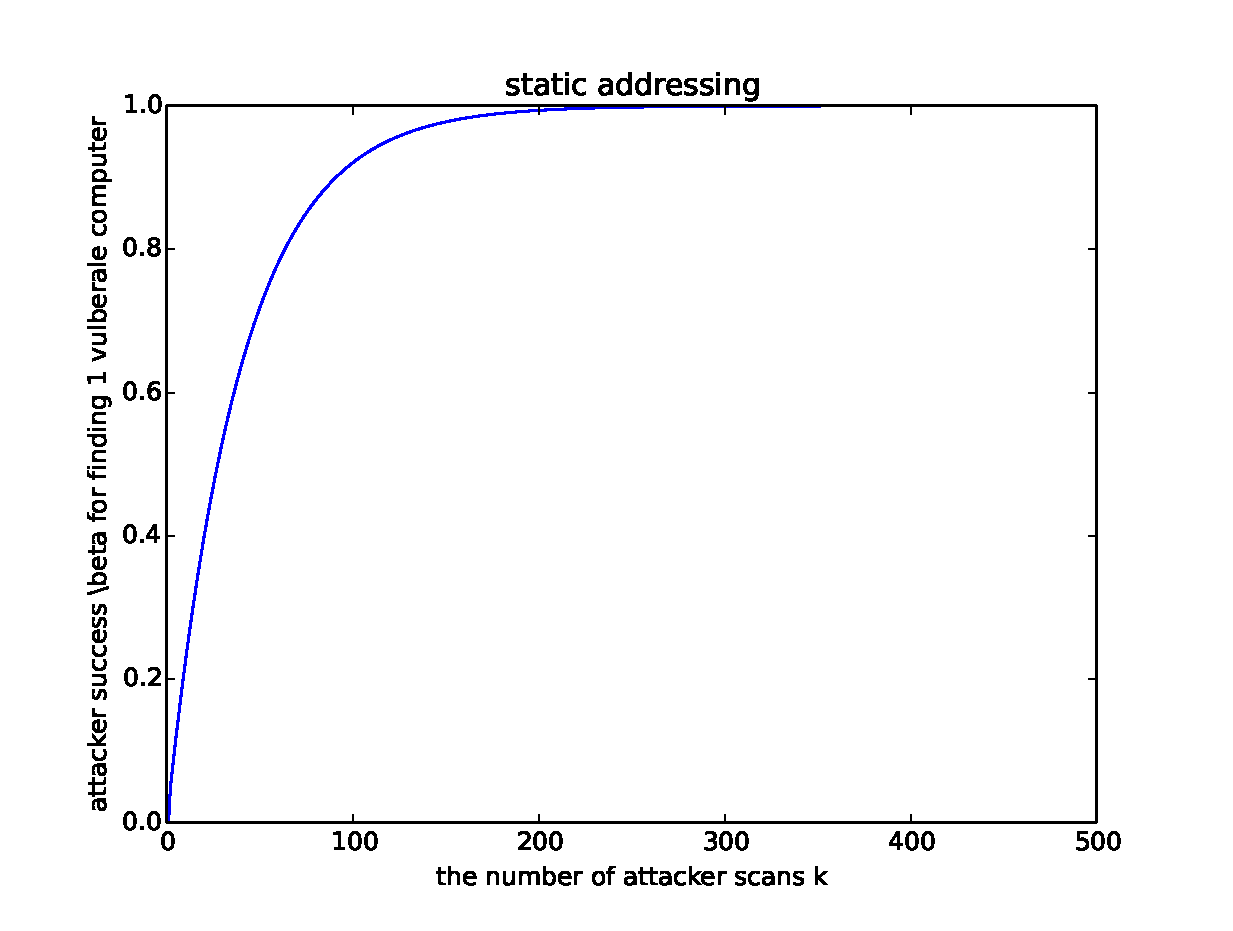
\includegraphics[width=0.8\textwidth]{figure1.2.eps}
\caption{Plot of question 1.2, static addressing}
\end{center}
\end{figure}

From the figure above the attacker will almost always find the first vulnerable computer successfully within about $200$ scans, that's because the total vulnerable computers are $\frac{1}{40}$ of the whole IP addresses space, the average scans the attacker need to find the first vulnerable computer is $40$, thus with more than $200$ scans could almost guarantee the attacker find at least one vulnerable machine.

\subsubsection*{1.3}

Still, using Python we have the attacker success rate $\beta$ as the number of scans $k$ and attacker find percentage $\alpha$ increases:

\begin{figure}[H]
\begin{center}
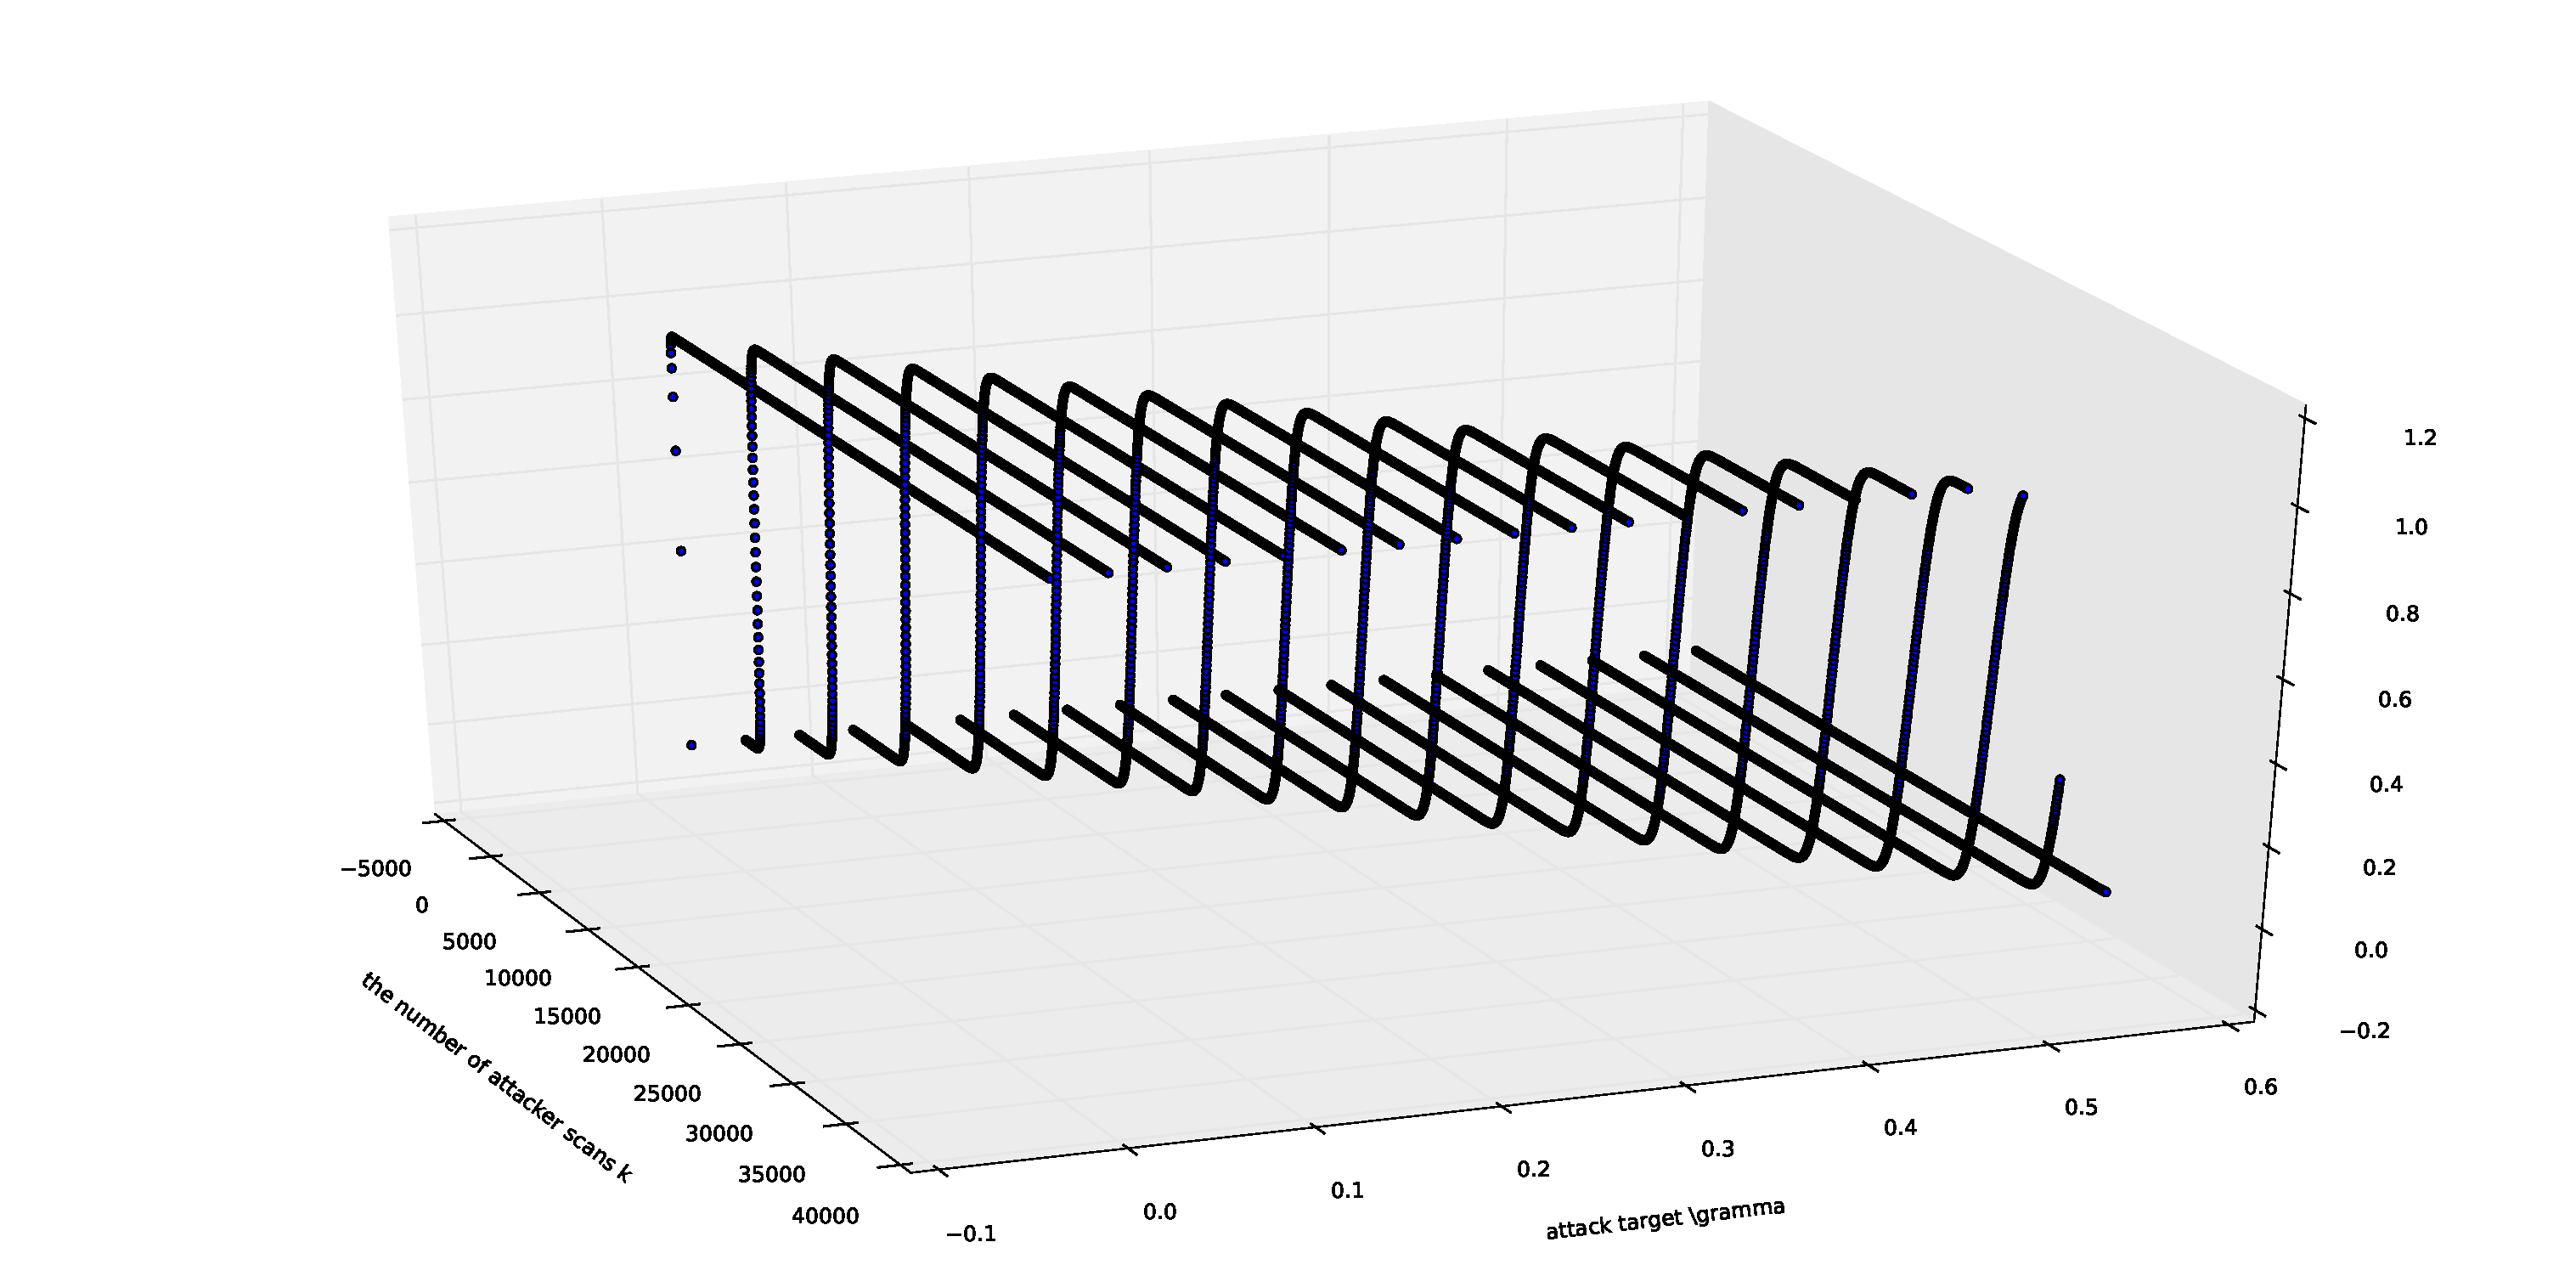
\includegraphics[width=0.8\textwidth]{figure1.3.eps}
\caption{Plot of question 1.3, static addressing}
\end{center}
\end{figure}

As we can see here, with the attacker find percentage $\alpha$ increasing, the attacker needs more and more scans $k$ to achieve a higher attack success. But when the attacker find percentage $\alpha$ becomes too high, say over $60\%$, then it is just too hard to achieve a acceptable attack success $\beta$, that's will require a significant big number of scans. \\
// which is very similar to the accomplishment of this project, if one (like, me) wants to finish $100\%$ of it, // it's nearly impossible within :) \\
(Note: the paragraph above is commented out such that no one can read it unless he failed an inverse Turing Test).


\subsubsection*{2.1}

For the perfect shuffling where $\gamma = 1$, now we have $k$ shuffles, each shuffle after each scan. Here, we want to point out that for each successful scan (that the attacker find a vulnerable machine) the attacker makes, it's possible that the attacker could find the same vulnerable machine with what he found before, when this situation occurs, we assume that the attacker will view this as a new vulnerable machine, this is not only for the simplicity of building up models, but also for the fact that when the Id address space $n$ is big enough, the possibility that the attacker find "enough many" same vulnerable machines is very small so that we can afford to omit it.


Using the same analog we stated in the question $1.1$, the naughty boy will play the "seeking for red candies" game $k$ times, but instead of picking all $k$ boxes at the same time in one game, he will pick only one box at each one game and he is given $n$ brand new boxes at each game. Since the number of red candies at each game are always $v$, thus the possibility of the boy gets a red candy at each game is $\frac{v}{n}$, then the possibility that he get $x$ red candies in those $k$ games is $k \choose x$$(\frac{v}{n})^x(1-\frac{v}{n})^{k-x}$. Still, at least $\alpha v$ red candies can make him happy, thus:
\beq
\beta &=& \sum\limits_{x=\alpha v}^{\min{(k,v)}} {k \choose x}(\frac{v}{n})^x(1-\frac{v}{n})^{k-x}. \nonumber
\eeq

\subsubsection*{2.2}
Here, $n = 2^{16}-2 = 65534$, $m=\frac{n}{4} = 16383.5$, $v = \frac{m}{10} = 1638.35 \doteq 1639 $ and $\alpha v = 1$. In order to compare its graph with static addressing, I plot both curves in the graph using Python, as follows

\begin{figure}[H]
\begin{center}
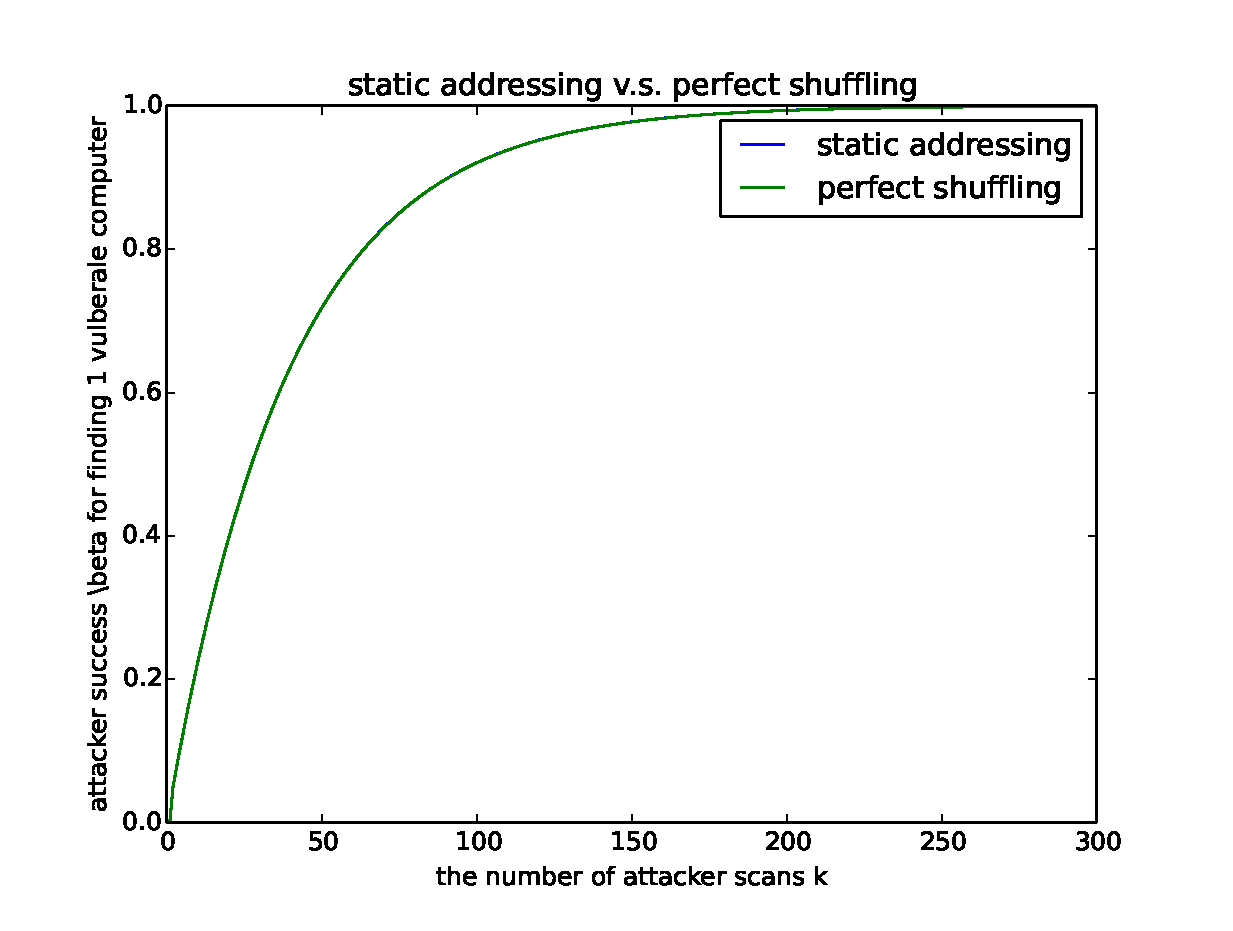
\includegraphics[width=0.8\textwidth]{figure2.2.eps}
\caption{Plot of question 2.2, using address shuffling strategy }
\end{center}
\end{figure}

As we can see that, those two curves are overlapped, can't really tell a differences visually. But deep inside we tend to believe that perfect addresses shuffling should do slightly better than static address (in terms of decreasing the attacker success given the same scans), otherwise our effort is in vain and there will be no point of calling this method a "defense". Theoretically, the attacker is playing the game without replacement, the possibility that he to get a vulnerable machine at the $k$th scan is depending on his previous "$k-1$" scans. While under perfect shuffling strategy, the attacker is playing $k$ independent games, that his posteriori scans will not be affected the results of his prior scans. Thus, as the scans $k$ becomes bigger, the difference between those two methods should become more obvious:

\begin{table}[H]
\begin{center}
\begin{tabular}{| c || c | c || c | }
  \hline
$ scans k $&$ static-address(S)$&$perfect-shuffling(P)$&$ winner$
\\  \hline
$50$&$ 0.72512198370323211 $&$ 0.72506160021762656 $&$ P $
\\  \hline
$70$&$ 0.83439473355419358 $&$ 0.8342980136319853 $&$ P $
\\  \hline
$100$&$ 0.92258098492144669 $&$ 0.92247064238466114 $&$ P $
\\  \hline
$150$&$ 0.9782164209012405 $&$ 0.97813764357046307 $&$ P $
\\  \hline
$\vdots$&$ \vdots $&$ \vdots $&$ P $
\\ \hline
\end{tabular}
\end{center}
\caption{Comparison of static address and perfect shuffling given bigger scans $k$ .}
\label{VerifyJ}
\end{table}


\subsubsection*{2.3}

With shuffling frequency $\gamma$, then we will perform $\gamma k$ shuffles during the attacker's $k$  scans, thus we will perform one shuffle after $\frac{k}{\gamma k} = \frac{1}{\gamma}$ scans.
During each $\frac{1}{\gamma}$ scans before the next shuffling, the possibility that the attacker will get $x$ vulnerable computers is: $\frac{{v \choose x}{n-v \choose \frac{1}{\gamma}-x}}{{n \choose \frac{1}{\gamma}}}$, thus the final total number of the vulnerable computers the attacker can get in the end is the sum of those $x_i$s ($0 \leq i \leq \gamma k$) from each $\frac{1}{\gamma}$ scans, then the attacker success $\beta$ is:
\beq
\beta &=&\sum \limits_{x_{\gamma k} =0}^{\min{(k,v,\frac{1}{\gamma})}} \ldots \sum \limits_{x_{2}=0}^{\min{(k,v,\frac{1}{\gamma})}} \sum\limits_{x_{1} =0}^{\min{(k,v,\frac{1}{\gamma})}} \prod\limits_{i=1}^{\gamma k} \frac{{v \choose x_i}{n-v \choose \frac{1}{\gamma}-x_i}}{{n \choose \frac{1}{\gamma}}}, where \sum\limits_{i=1}^{\gamma k} x_i \geq \alpha v \nonumber
\eeq


\subsubsection*{2.4}

It's toooooo hard to plot this one :(

When I showed my equation in $2.3$ to you Monday afternoon, you said forgot about it ...


\subsubsection*{2.5}
Shuffling the entire network provide more protection. In the equation of question $2.3$, only shuffling vulnerable machines with empty addresses will make the denominator smaller, hence the attacker success will become bigger, thus shuffling the entire network is better.


\subsubsection*{3.1}

For each subnet $i$, $1 \leq i \leq s$, suppose the attacker also performs $y_i$ scans, thus $\sum\limits_{i=1}^{s} y_i = k$. Since it's perfect shuffling $\gamma=1$, the whole subnets shuffl after each scan. Thus the possibility that the attacker find a vulnerable with each scan at each subnet is still $\frac{v/s}{n/s} = \frac{v}{n}$. Also also, suppose the attacker will get $x_i$ vulnerable computers from the $i$th subnets within $y_i$ scans, we have

\beq
\beta &=&\sum \limits_{x_s=1}^{\min{(y_s,\frac{v}{s})}} \ldots \sum \limits_{x_{2}=0}^{\min{(y_2,\frac{v}{s})}} \sum\limits_{x_{1} =0}^{\min{(y_1,\frac{v}{s})}} \prod\limits_{\sum\limits_{i=1}^{s} y_i = k}^{i=1\ldots s} \frac{{\frac{v}{s} \choose x_i}{\frac{n-v}{s} \choose y_i-x_i}}{{n \choose y_i}}, where \sum\limits_{i=1}^{s} x_i \geq \alpha v \nonumber
\eeq

\subsubsection*{3.2}

When $s$ is small enough, this plot is quite similar to question $2.2$. (The reason why $s$ can't be too big will be further addressed in question $3.3$.) Because no matter how the defender is diving the network into subnets and do shuffling, there is not making much differences to the attacker, and the attacker may not even be aware of this.

\begin{figure}[H]
\begin{center}
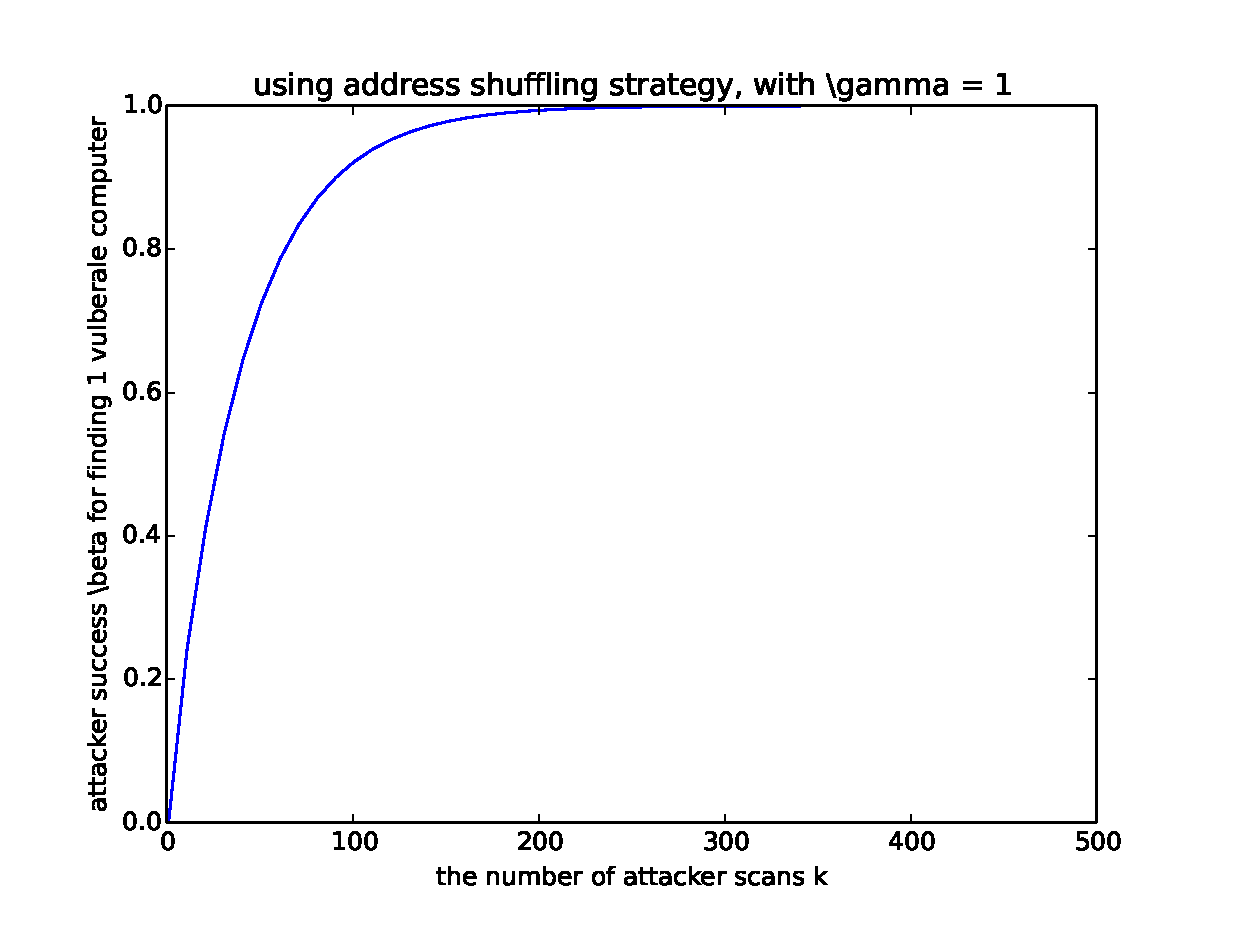
\includegraphics[width=0.8\textwidth]{figure2.2.orginal.eps}
\caption{Plot of question 3.2, using D-Quan's address shuffling strategy }
\end{center}
\end{figure}


\subsubsection*{3.3}
From my point of view, I think the method is worse or no better than the traditional shuffling. Let's consider an extreme example, that when $s$ is too big, say $s=2^8$, then with a $\setminus 16$ (class B) network, you are going to get $\frac{2^16}{2^8}=2^8$ subnets (class C), now the total available IP addresses are $2^8\times(2^8-2)=2^16-2^9$, while originally we have $2^16-2$ available IP addresses, this diving leads to $2^9-2$ less than original IP addresses space, which make the denominator of the attacker success equation small, hence make the attacker success $\beta$ bigger.


\subsubsection*{4.1}

In this question, there is one situation that, the attacker could achieve his success (by finding $\alpha v$ vulnerable machines) without contacting any honeypots (yes, he is lucky) before using up all the $k$ scans, then this occurs, we assume that he will continue scanning until finishing his $k$ scans, during this process he could gain more vulnerable machines but also he may contact honeypots, in this situation we will view this as a failure even though he already got enough vulnerable machines, because he is caught (never be too greedy). 

Now, first of all, we want to know the possibility that the attacker performed $k$ scans without contacting any honeypots:
\beq
P(k-scans-without-honeypots) &=&\frac{{n-h \choose k}}{{n \choose k}}. \nonumber
\eeq
Thus,
\beq
\beta &=& P(find-\alpha v-vulnerable computers|k-scans-without-honeypots)P(k-scans-without-honeypots)\nonumber \\
&=&  \sum\limits_{x=\alpha v}^{\min{(k,v)}} \frac{{v \choose x}{n-h-v \choose k-x}}{{n-h \choose k}}\frac{{n-h \choose k}}{{n \choose k}} \nonumber \\
&=&  \sum\limits_{x=\alpha v}^{\min{(k,v)}} \frac{{v \choose x}{n-h-v \choose k-x}}{{n \choose k}}. \nonumber
\eeq

\subsubsection*{4.2}

Here, $n = 2^{16}-2 = 65534$, $m=\frac{n}{4} = 16383.5$, $v = \frac{m}{10} = 1638.35 \doteq 1639$, $\alpha v = 1$ and $k = \frac{n}{10} = 6553 $, in Python we have:


\begin{figure}[!htb]
\begin{center}
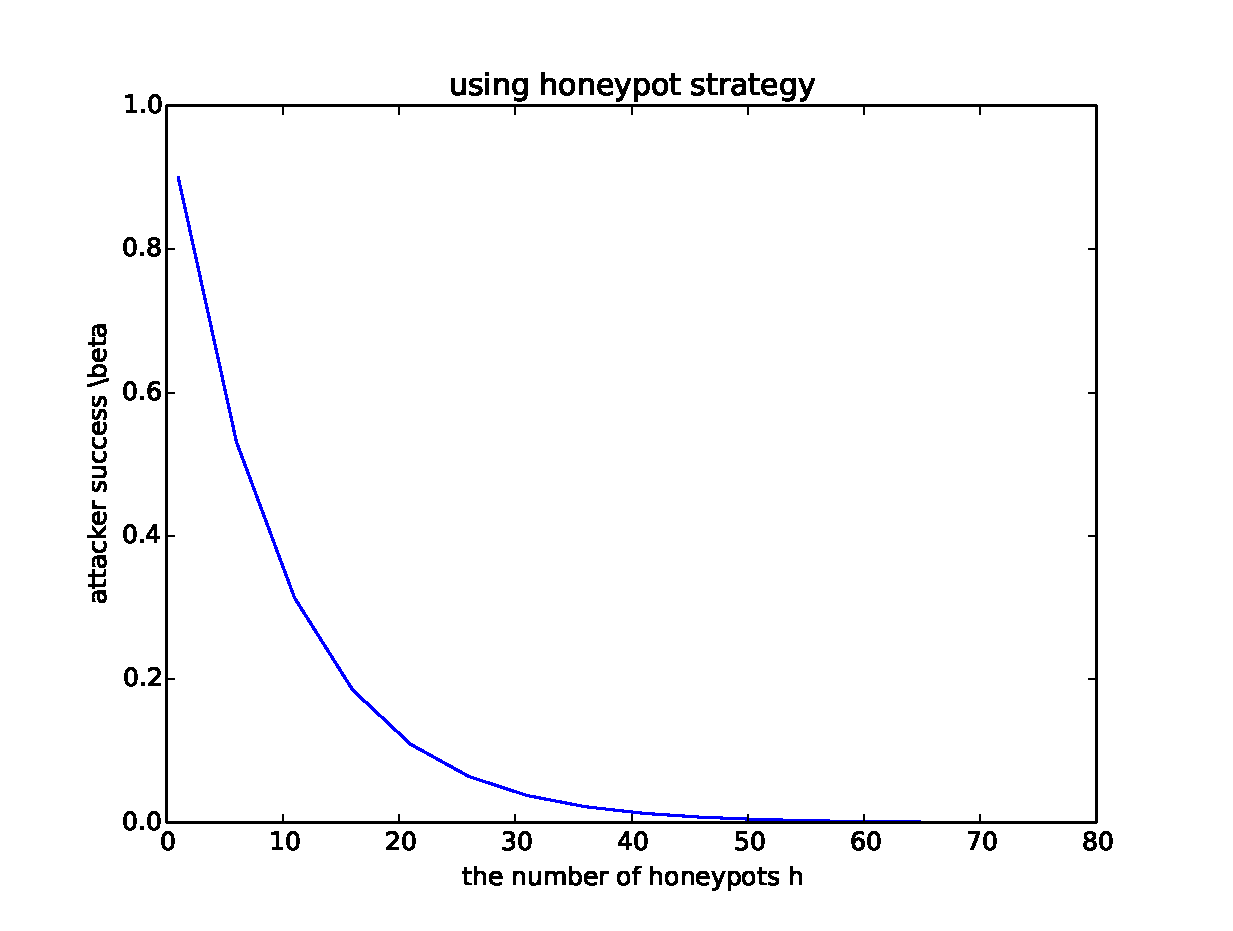
\includegraphics[scale=.7]{figure4.2.eps}
\caption{Plot of question 4.2, using honeypot strategy }
\end{center}
\end{figure}

%\begin{figure}[!htb]
%\centering
%\includegraphics[scale=.7]{nfa.eps}
%\caption{Digraph.}
%\label{fig:digraph}
%\end{figure}

With the $k=6553$ scans, from the result of Figure $3$ in question $2.2$, we know that the attacker will almost necessarily find at least one vulnerable machine. But with the number of hoenypots increasing, the attacker would be less likely to avoiding contacting honeypots. When the number of honeypots is big enough, say great than $60$ as we can tell from the graph, the attacker will almost necessarily to fail if he insist to finish all the scans. 


\subsubsection*{4.3}

Using Python we have:

\begin{figure}[H]
\begin{center}
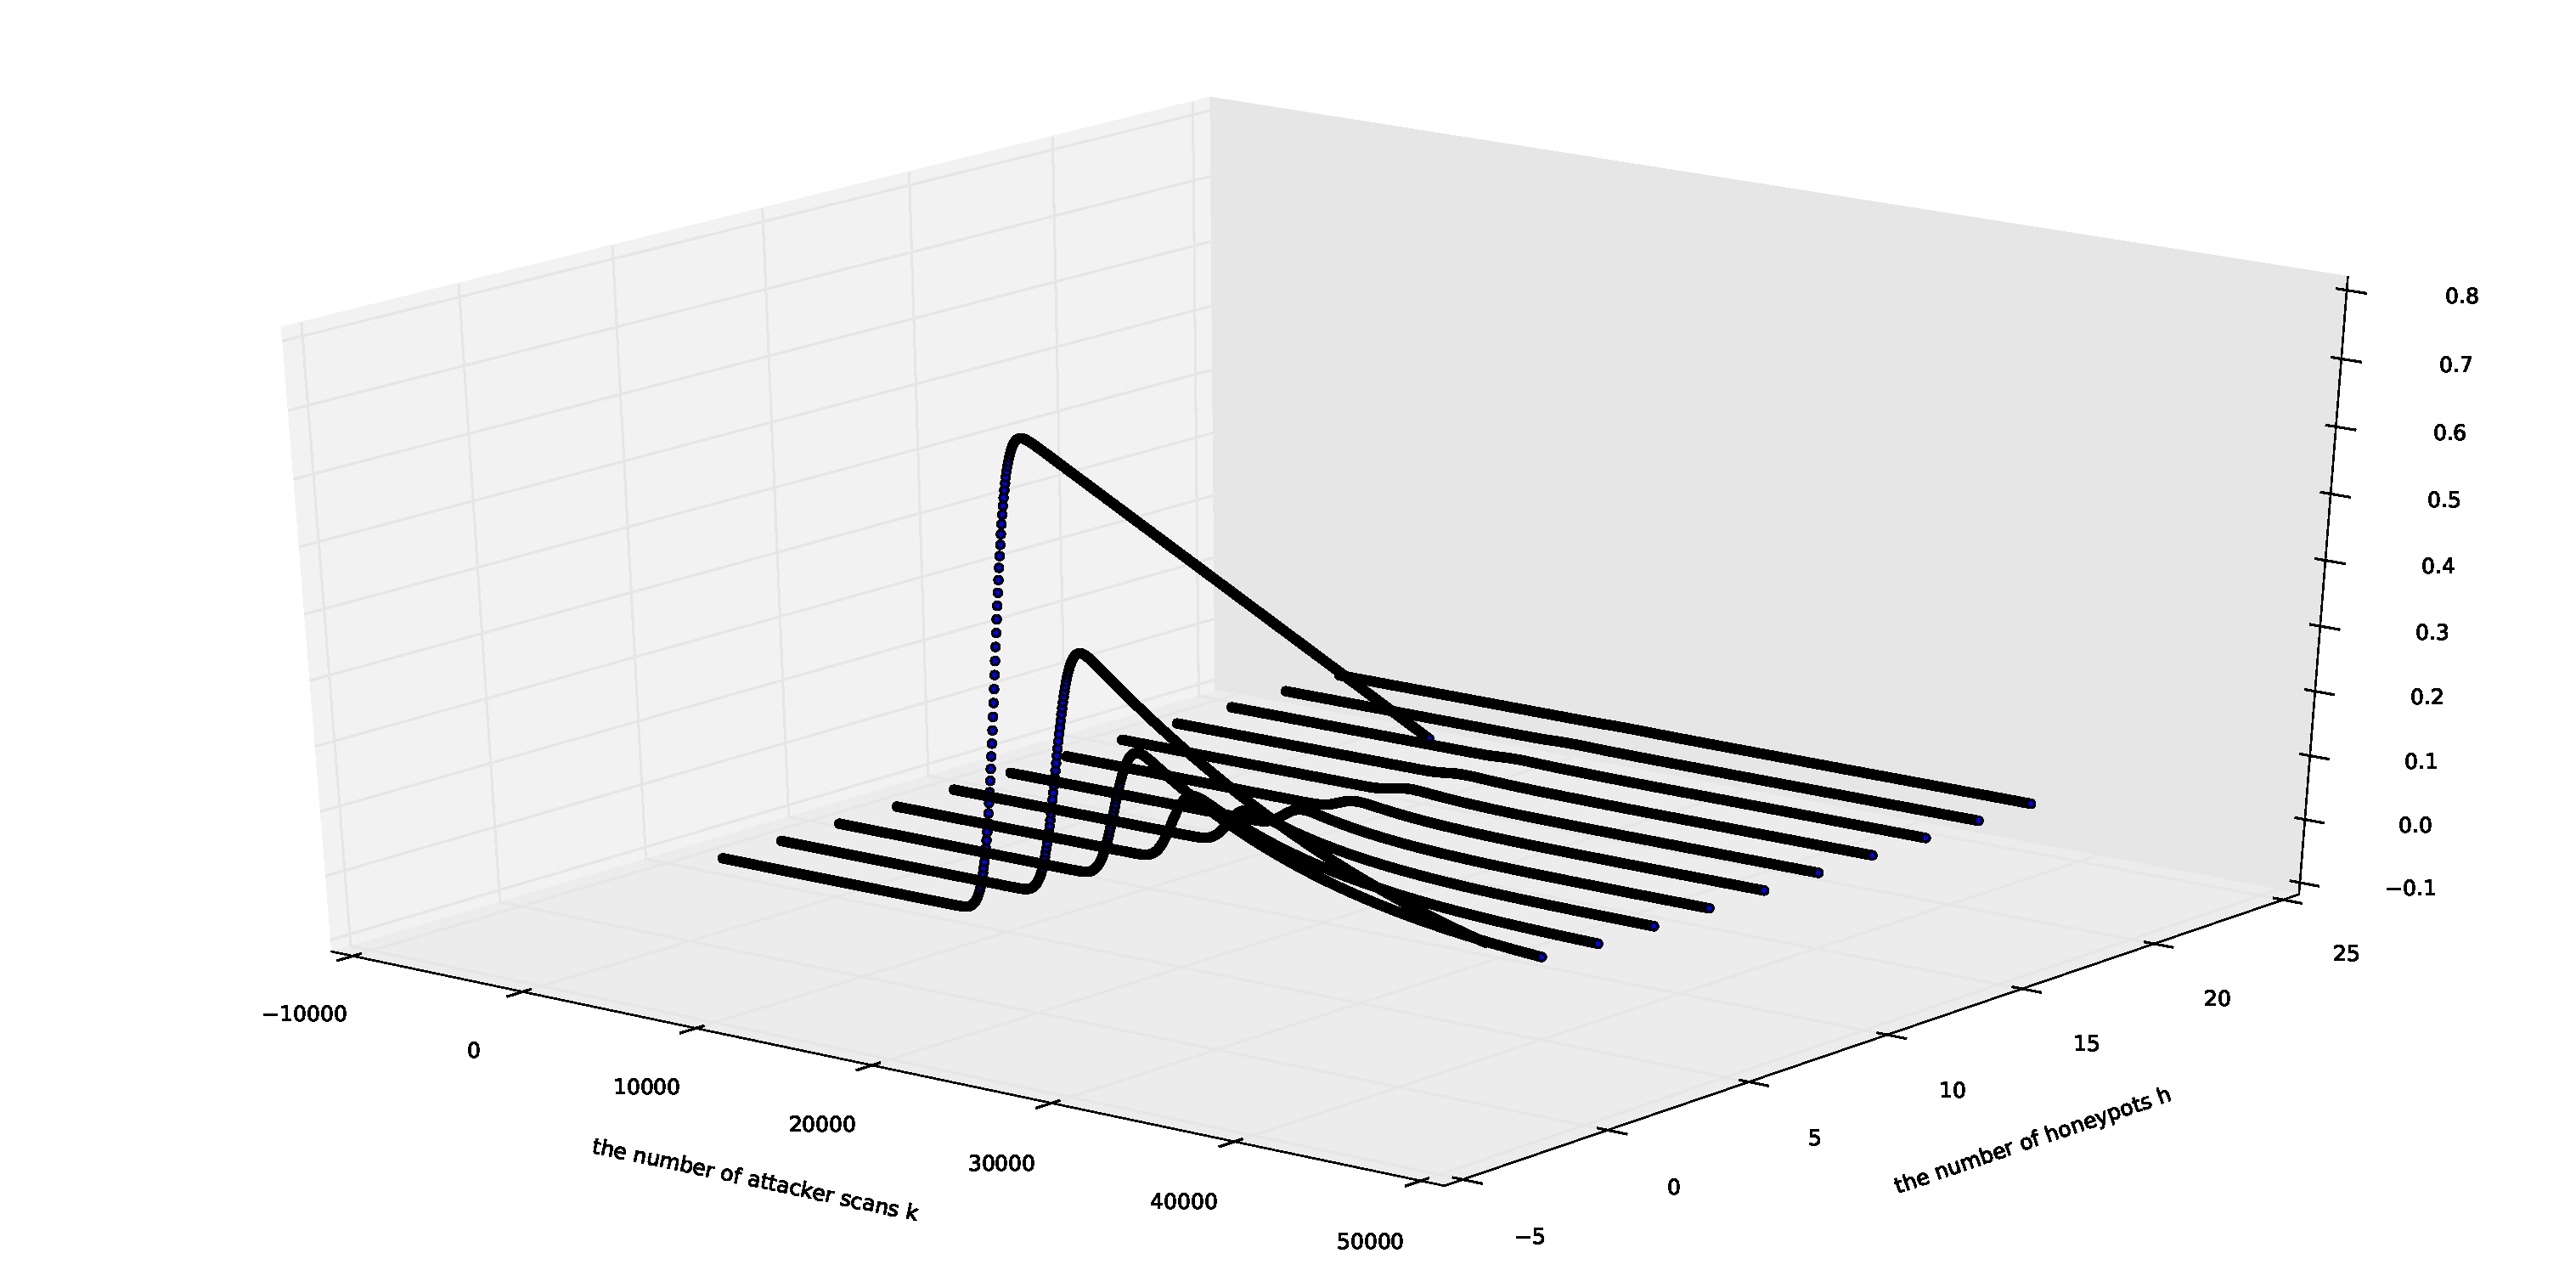
\includegraphics[width=0.8\textwidth]{figure4.3.eps}
\caption{Plot of question 4.3, using honeypot strategy }
\end{center}
\end{figure}

Since it is require and find at least $25\%$ of the vulnerable machines, from question $2$ we know that attacker need a significant many scans to accomplish this (somewhere above $20,000$ ). But with the numbers of honeypots increases, it's harder and harder and finish those scans without contacting any honeypots, as you can see from the graph above, the attacker success $\beta$ approaches to $0$ when there are more than $20$ honeypots deployed. 


\subsubsection*{5.1}

The defender side: \\
\indent revenue:  \\ 
\$1000 per win using any strategies \\
\indent cost: \\
\$2000 per lose \\
no cost using static address \\
\$5 per shuffling using addresses shuffling address strategy \\
\$100 per honeypot deployment using honeypots strategy \\ \\

\noindent The attacker side: \\
\indent revenue:  \\
\$2000 per win  \\
\indent cost: \\
\$1000 lose per lose \\
\$50 per honeypot deployment using honeypots strategy \\



\subsubsection*{5.2}

Suppose a $\setminus 8$ (class C) network, with $100$ machines and 20 of them are vulnerable, given a attacker wants to scan $k=50$ scans to get at $25\%$ of the vulnerable machines, which is 5. Now consider the attacker success $\beta$:

For static addressing:
\beq
\beta &=& \sum\limits_{x=5}^{20} \frac{{20 \choose x}{254-20 \choose 50-x}}{{254 \choose 50}} \nonumber \\
&=& 0.35
\eeq

For perfect shuffling:
\beq
\beta &=& \sum\limits_{x=5}^{20} {50 \choose x}(\frac{20}{254})^x(1-\frac{20}{254})^{50-x} \nonumber \\
&=& 0.35. \nonumber 
\eeq

For honeypots:
\beq
\beta &=&  \sum\limits_{x=\alpha v}^{\min{(k,v)}} \frac{{v \choose x}{n-h-v \choose k-x}}{{n \choose k}}. \nonumber \\
\eeq
We have: 
\beq
\beta &=& 0.28 , where h=1 \nonumber \\
\beta &=& 0.23 , where h=2 \nonumber \\
\beta &=& 0.18 , where h=3 \nonumber \\
\beta &=& 0.14 , where h=4 \nonumber \\
\beta &=& 0.12 , where h=5 \nonumber \\
\eeq

Based on those costs and revenues we assigned above, we have the expected income for the defenders is that:
\beq
E(static) &=&  (1-0.35)\times 1000 + 0.35\times(-2000)\nonumber \\
&=& -50 \nonumber \\
E(perfect-shuffling) &=& (1-0.35)\times 1000+0.35\times(-2000)-50\times5 \nonumber \\
&=& -300 \nonumber \\
E(honeypots|h=1) &=& (1-0.28)\times 1000+0.28\times(-2000)- 100  \nonumber \\
&=& 60 \nonumber \\
E(honeypots|h=2) &=& (1-0.23)\times 1000+0.23\times(-2000)- 100 \times 2 \nonumber \\
&=& 110 \nonumber \\
E(honeypots|h=3) &=& (1-0.18)\times 1000+0.18\times(-2000)- 100 \times 3 \nonumber \\
&=& 160 \nonumber \\
E(honeypots|h=4) &=& (1-0.14)\times 1000+0.14\times(-2000)- 100 \times 4 \nonumber \\
&=& 180 \nonumber \\
E(honeypots|h=5) &=& (1-0.14)\times 1000+0.14\times(-2000)- 100 \times 5 \nonumber \\
&=& 140 \nonumber \\
\eeq

More honeypots will definitely improve more defence, but deploying honeypots are also very expensive. In our example, we decide to deploy $4$ honeypots to maximize our revenue. 

\end{document}
